
\section{WORKBOOK LESSON 2
CHART JUDGMENT}
 

The following are important summary rules on chart judgment. You should try to keep these in mind as much as possible. Some of them repeat the basic information given in the previous lesson but in a different way. Bear in mind that this is material that you need to really memorize, so such repetition should be helpful.

 

Please study this Workbook Lesson along with Part I. Lesson 7, which also deals with the judgment of the horoscope with additional information.

 



 

\subsection{House Location of Natural Benefics and Malefics}
 

When giving an overall judgment of the chart first examine the house location of the planets by their natural status. The main rule is:

 

Natural benefics do best in angles or trines – 1, 4, 5, 7, 9, 10 \\
Natural malefics prefer upachaya houses    – 3, 6, 11\\
 

These rules also apply to divisional charts. It is a particularly important rule for noting the overall health and longevity of the person.

The correlation that must be borne in mind is that all planets do better in signs that they rule or signs in which they are exalted. But even these good positions are compromised by location in difficult houses. Similarly difficult planets do better in signs they rule or signs in which they are exalted even if these difficult placements.

 

\subsubsection{NATURAL BENEFICS}
 

\paragraph{In Angles and Trines}

 

Natural benefics (Jupiter, Venus, Mercury, Moon) do best in angles (4, 7, 10) or in trines (1, 5, 9). However, benefics when retrograde do not always give their benefits and become unpredictable (though they are not harmful). Benefics in angles are more weakened by retrograde status than are those in trines. Debilitated benefics in angles and trines will also prove uncertain but still overall prove helpful unless badly aspected. The same is true of a weak and waning Moon or a badly associated Mercury, which may not give good results by a good house position.

 

\paragraph{Angles}

The tenth is the strongest angular position for benefics followed by the seventh, fourth and first. However, the seventh is good mainly for career. Benefics here can harm marriage by making the person too quick to get into relationships. Sometimes benefics in the seventh can harm health (the seventh being a maraka house; note more information below).

 

Benefics in their own signs or exalted in angles create Mahapurusha Yogas, which have been discussed (like Mars in Aries in the tenth house). These serve to mark the character and physical type of the person and can greatly elevate a person in life.

 

Angular locations for benefics may not always confer spiritual benefits however, but will be helpful in the worldly sense. After all the angles reflect more the outer side of our nature. Generally planets in angular positions are stronger than in trine positions.

 

\paragraph{Trines}

The ninth is the best trine followed by the fifth and first. The ninth elevates us and gives us good values, good luck and a good future. The fifth gives us good karma and a good mind. Trine locations are usually beneficial both spiritually and materially. Generally the ninth gives more favor from parents, teachers, gurus, schools, institutions and the government. The fifth gives merit to oneself, good samskaras (past life-tendencies), and a good intelligence. It also gives happiness through children and creative work like writing depending upon its disposition. Jupiter does better in trines than other benefics because of its trinal aspects, which will always aspect the Ascendant.

 

\paragraph{In Duhsthanas}

Benefics suffer in Duhsthanas (6, 8, 12) in which their good powers are wasted and they can cause harm, particularly disease, by their weakness. From their position in the sixth disease, enemies and conflict increase. In the eighth house sudden obstacles, disease, financial losses and accidents arise. In the twelfth loss of fame, weakened vitality, wrong generosity, and time in hospitals, prisons, or retirement from life is likely.

 

Benefics in the eighth and twelfth, however, can be good for spiritual matters, particularly unafflicted Mercury or Jupiter, and especially if conjoined with Ketu. The same is true of these planets in the fourth house, another Moksha house, and unafflicted. Such positions give occult and spiritual insight. Benefics in the twelfth are also good for travel, for living overseas, and for dealing with foreign countries, peoples and cultures, in which case they may not bring much trouble. The Moon tends to suffer more in these positions than the other benefics and is a position for weak health or poor constitution.

 

In the Second, Third and Eleventh Houses Benefics suffer to a lesser degree in the third house, which is eighth from the eighth. In the third they create desire but also talent and artistic ability. They also bring benefit to ones siblings.

 

Benefics generally do well in the eleventh house, however, in which house all planets are generally good. The eleventh gives abundance to whatever planet is located there. It is good mentally and, of course, financially, being the house of gain.

 

Benefics in the second house are good for self-expression and for business but not always for health (the second being a maraka house).

 

\paragraph{Own Sign and Exaltation}

Location of a planet in its own sign or sign of exaltation improves the status of benefics in bad houses but does not eliminate it. For example, an exalted Jupiter in the sixth house can still cause health problems, though less than otherwise. However it will be good for its own houses, two and eleven, increasing wealth.

 

Location in its own sign or sign of exaltation greatly improves the power of benefics located in good houses, of course creating a Mahapurusha Yoga.

 

However, a benefic in its own sign under affliction causes a house to be doubly harmed. In this instance both the house and its lord suffer, even if the house is good. For example, the Jupiter in the tenth house aspected by Saturn and with Rahu, may cause too much public expansion leading to a great fall, controversy, or litigation.

 

\paragraph{House Location of Natural Benefics}

 
\begin{center}
\begin{tabular}{ c c  }
Positive & 1, 4, 5, 9, 10, 11 \\ 
Mixed & 2, 7 \\  
Negative & 3, 6, 8, 12   
\end{tabular}
\end{center}



\paragraph{Temporal Benefics and Malefics}

 

Generally natural benefics improve the houses they occupy, even if these are difficult houses, but they also weaken the houses that they rule. For example, if Jupiter is located in the twelfth house in Libra, it may help the eighth house to some degree, but it will not be good for the houses that it rules (in this case the second and the fifth houses). In addition, the ability of Jupiter to provide good results will be limited by its position in the eighth house. Of course, its aspects on other houses and planets must also be considered.

 

If a planet is a natural benefic but a temporal malefic, like Jupiter ruling the third and sixth for Libra Ascendant, its natural benefic status and influence will be compromised, though not entirely eliminated. For a complete reading of the chart we should look into the temporal status as well.

 

\subsubsection{NATURAL MALEFICS}
 

\paragraph{Upachaya Houses}

 

Natural malefics (Saturn, Mars, Rahu, Ketu, Sun) do best in upachaya houses (3, 6, 11). Here they guard the health of the person and are a source of strength, vitality and motivation, and give the capacity to do hard work. Malefics in upachaya houses give a person steadiness, fearlessness, courage and the ability to make great achievements. Sometimes the tenth house is also counted as an upachaya house particularly for Mars, the Sun and Rahu.

 

The exception is that more than one malefic in the sixth, or a malefic in the sixth under malefic aspect, can cause health problems. Generally the eleventh is the best house for malefics. Yet even in these houses the aspects of malefic planets can cause harm to other aspects of a persons life and relationships. For example, Saturn in the eleventh will still cast an aspect on the fifth that can be harmful for children, though it will give a person the ability to succeed in their long term personal ventures.

 

\paragraph{Angles and Trines}

Natural malefics in angles and trines (1, 4, 5, 7, 9, 10) usually cause harm and suffering. Without any benefics in angles and trines to counter their influence, malefics in these positions can cause great harm to a person, including major health problems or injury.

 

In angles malefics may give success, particularly if they rule good houses or are in a good sign position. Yet they tend to make the person harsh, of bad character, or difficult to deal with. They can give one powerful enemies even if they make a person strong himself. For example, Mars in Aries in the tenth house will be good for success but can cause some degree of enmity or make the person aggressive in temperament. Mahapurusha Yogas give greater strength to malefics for power and success but do not always give a better character or spiritual life. Saturn becomes strong in the seventh house and Mars in the tenth because of their aspects to the Ascendant from these positions.

 

In trines malefics are generally harmful, damaging these good houses.  Malefics in trines harm our good fortune. For example, in the fifth they harm children or weaken ones intelligence, and in the ninth they harm the father or cause trouble with education or the government. Malefics in the fifth can weaken the health. But overall malefics in trines are not as bad as malefics in angles.

When retrograde in angles and trines, malefics can cause yet more harm. When debilitated, malefics cause less harm but also confer less power upon the person. In fact debilitated malefics can make a person humble or spiritual because the pride of the malefic is weakened.

 

The Sun, however, generally does well in the tenth house and does not suffer as much from location in an angle. The Sun in the first and tenth house can give a person a strong character and charisma.

 

In the seventh house, on the other hand, the Sun is particularly difficult for relationship though it can be good for career. The Sun in the seventh can be worse than Mars and can cause relationships with people who are already married. The Sun can be difficult in the fifth house and delay or deny children.

 

Mars gains directional strength in the tenth and so is not entirely negative there either. Saturn gains directional strength in the seventh but is only good there for career, not for relationship, either limiting relationship capacity, causing detachment or creating perversions. Saturn in the tenth can be very strong to raise a person up but also leads them to a fall. Generally malefics in the tenth give power which leads to an excess that causes harm.

 

\paragraph{Temporal Lordship}

When good temporal lords, malefics in angles and trines give better results, particularly for worldly matters. This is especially true if the planets are yoga karakas. For example, Mars in the tenth in Taurus gives success because it is a yoga karaka (ruler of the fourth and ninth) for Leo Ascendant. However, the strongly placed Mars may make the person harsh or obstinate. The effects of planets on houses should be judged by their temporal status as well as by their natural status.

 

Generally the effects of malefics in angles will outweigh that of benefics, should both types of planets be angular in the chart. The factor should always be borne in mind.

 

\paragraph{Duhsthanas and Other Houses}

Malefics in Duhsthanas (6, 8, 12) are also weak, with the exception of the sixth as already noted, which as an upachaya house makes them strong. Saturn in the eighth can be good for health or longevity but may otherwise cause trouble financially or in terms of career and relationship. Saturn retrograde or afflicted in the eighth can cause harm to the health as well. Malefics like Saturn in the twelfth can be good spiritually, however, because they show renunciation of the comforts of life. Malefics in Duhsthanas generally weaken our energy and vitality.

 

Malefics in the second house usually cause harm, both to the speech of a person and to their happiness in childhood. Mars here gives a person sharp, aggressive or clear speech. Saturn gives detachment or poverty.

 

\paragraph{Rahu and Ketu}

Rahu and Ketu are exceptional in that they usually do well in the six-twelve axis, particularly Rahu in the sixth and Ketu in the twelfth, in which the Moksha or liberation giving power of Ketu becomes strong. They can still cause difficulties in these houses but such difficulties will be overcome or lead to greater accomplishments. For example, Rahu in the sixth gives enemies and diseases but one overcomes them.

 

Rahu in an angle associated with a Lord of a trine or in a trine associated with a Lord of an angle gives Raja Yoga and is very good. For example, Rahu in the tenth house in Cancer (Libra Ascendant) along with Mercury (ninth lord) would give Raja Yoga. Do not ignore this type of Raja Yoga. Some also count Rahu in trine with its lord in an angle as a similar Raja Yoga.

 

Otherwise Rahu and Ketu do better in upachaya houses like other malefics. But care must always be taken to look at their dispositors, which determine greatly how they function. Generally natural malefics harm the houses that they occupy.

 

\paragraph{House Location of Natural Malefics}


 
\begin{center}
\begin{tabular}{ c c  }
Positive & 3, 6, 11 \\ 
Mixed & 7, 10 \\  
Negative & 1, 2, 4, 5, 8, 9, 12  
\end{tabular}
\end{center}
 

\subsection{House Lords }


After examining the natural status of the planets in the chart, one must also look at their temporal status by house rulership. This is more difficult and more intricate but is necessary for a full examination. Most complicating is the fact that planets (except Sun and Moon) will rule two houses in the chart, one of which may be a good house and the other a difficult house. The planet will give the results of both houses depending upon the influences upon them.

 

These houses cover all the domains of life from personal health, well-being and success, to relations like father, mother, brothers, sisters and children, to outer factors like houses, vehicles, wealth and adornments, and inner factors like spirituality and Yoga practice. Blending all these house considerations is the essence of Vedic astrology.

 

\subsubsection{Raja Yoga/ Trinal Lords}

 

Lords of angles and trines do better in association with each other in the chart, in which case they give Raja Yoga, particularly if their combination occurs in angular or trine houses. Yet a Raja Yoga occurring in difficult houses (6, 8, 12) will still confer some benefit. However it may require overcoming an obstacle, being first defeated, or undergoing humiliation before ones success.

 

A lord of a trine remains generally benefic, even if the other house the planet rules is not a benefic house. If its other house is two or twelve it remains mainly benefic (like Venus for Gemini and Virgo Ascendants). If its other house is six or eight, it will also cause some harm to the person, particularly in terms of health, but still do good (like Saturn for Gemini and Virgo Ascendants).

 

Generally the status of the Mulatrikona sign ruled by the planet will have more weight in making it benefic or malefic. For example, in the case of Virgo Ascendant, Saturn will ruler the fifth, Capricorn, and the sixth, Aquarius. As Aquarius is its Mulatrikona sign, it will tend to function more as the sixth lord.

 

\subsubsection{Maraka Planets}

 

Maraka (death-causing) planets are the lords of the second and seventh houses (as also planets located in these houses in the individual chart). These houses being twelfth from the houses of longevity (three and eight), serve to negate the life-giving qualities of these houses.

 

The second and twelfth houses from the Moon are also sometimes counted as Maraka houses.

 

Apart from these special maraka planets, the rulers of the eighth and twelfth houses have a maraka status, as well as natural malefics, particularly Saturn and Ketu.

 

\subsubsection{Ripening of Maraka Planets}

Maraka planets cause harm, not necessary death, to health only during the period of life in which their influence ripens.

 
\begin{enumerate}
\item If the chart is weak and indicates very poor health, their negative health effect can manifest during their Dashas in operation starting from the time of birth.
\item If the chart indicates average health, the negative effect of maraka planets will only manifest in their Dashas that occur after the age of 32, and can become critical after the age of 64.
\item If the chart indicates good health, the negative effect of maraka planets will only manifest in their Dashas that occur after the age of 64, and can become critical after the age of 80.
\item Otherwise maraka lords will give the ordinary results of the second and seventh houses, like wealth or marriage. But we should always examine them carefully.
\end{enumerate}


 

\paragraph{Maraka Planets and their Strength}

 

Maraka planets are more likely to cause harm when located in a maraka house (two and seven). Any planets in the second and seventh houses can become marakas.
Natural benefics can become maraka lords as well (like Jupiter for Gemini and Virgo Ascendants, or Mercury for Sagittarius and Pisces Ascendants). They cause trouble particularly when located in Duhsthanas (6, 8, 12).
 

 

\paragraph{Malefic Lords}

 

Lords of upachaya houses (3, 6 and 11) cause the most harm as malefic lords. The lord of the eighth causes harm but less so. The twelfth lord brings the least harm but does have a separative influence, removing us from what it influences. The lords of the eighth and twelfth usually combine with rulership of a more benefic house, giving them positive influence in other areas relative to the nature of the good houses that they also rule. Saturn for Gemini, for example, ruling Capricorn and Aquarius, the eighth and ninth houses, will give the results of both.

 

If a malefic lord is also an enemy of the Ascendant lord his malefic powers are increased (like Saturn for Cancer or Leo Ascendants). If he is a natural malefic his malefic power is increased yet further. If a malefic lord is a friend of the Ascendant lord his malefic powers are decreased (like Saturn for Virgo Ascendant).

 

\paragraph{Summary of Benefic Lords: Factors that increase benefic status}

 
\begin{enumerate}
\item Best: Lord of Both Angle and Trine, Raja Yoga Karaka
\item Second Best: Lord of trine but not an angle
\item Located in angle or trine house
\item Located in own sign, exalted or friendly sign, friend of ascendant lord
\item Natural Benefic
\item Not-retrograde
\item Similar conditions in divisional charts, particularly navamsha
\item In its own dashas, bhuktis and transits
\end{enumerate}

\paragraph{Summary of Malefic Lords: Factors that increase malefic status}

 
\begin{enumerate}
\item Lords of houses 3, 6, 11, 8 and 12, particularly if the other sign the planet rules is not a trine
\item Lords of 2 and 7 when their time has come
\item Located in angle, trine or Duhsthana house
\item Enemy of Ascendant Lord, in inimical sign
\item Natural Malefic
\item Retrograde
\item Similar positions in divisional charts, particularly navamsha
\item In its own dashas, bhuktis and transits
 \end{enumerate}

\subsubsection{Planetary Friendship and Enmity}
 

Planets do better when located in friendly signs and worse if located in unfriendly signs. This modifies (but does not entirely change) the indications of their house position. For this factor remember the rules of planetary friendship and enmity taught in the first part of this course, considering both the natural and temporal status of the planets.

 

Generally speaking 6-8 relationships are considered the most difficult, followed by 2-12. Positive or friendly relationships are mainly trinal (5, 9) and 3, 11 relationships. the others fall in between. These are counted from the house in which the planet in located in the chart. For example, if Jupiter is located in the fifth house in a chart but Saturn is located in the fourth house, then Saturn would be twelfth from Jupiter.

 

For example, a planet in the twelfth house in a friendly sign will suffer less than a planet in the twelfth house in an unfriendly sign, but it may not become entirely good either. It also does not negate mutual house positions. For example, planets in 2-12 house relationships are temporal friends but this still causes some difficulty by the inimical house relationship, particularly during their Dashas.

 

This factor also has an implication relative to house rulership. If a planet in a chart is located in the second, sixth, eighth or twelfth house from any house that it rules, the results of that house will be damaged. If it is located third, fifth, ninth or eleventh from the house that it rules, the results of that house will be improved.

 

\subsubsection{Priority of Factors}
 

1) House position generally has priority over sign position:

A planet located in its own, exalted or friendly signs but in a difficult house will still cause problems. Similarly a debilitated planet in a good house like a trine or angle will still give some good results. For example, a debilitated Jupiter in Capricorn in the ninth house will still give some good effects of the ninth house.

 

2) Malefic aspects can outweigh both good sign and good house positions:

Difficult aspects ruin good sign and house positions and can make them doubly negative. A benefic in an angle or trine under malefic aspects will not usually give good results but will show the good fortune of a person harmed or destroyed. For another example, a benefic in its own sign will be very much weakened by a malefic aspect.

 

3) Benefic aspects do not always outweigh bad sign and house positions:

A planet in a bad house will benefit by good aspects but the blemish of its bad location will not be entirely removed. For example, benefics in the sixth house will still suffer, even if they have some benefic aspects. Benefic aspects will show some help, like medical treatment of disease, but may not prevent the difficulty from arising.

In this regard consider house rulership as well. The aspect of a natural benefic but temporal malefic may not help a badly placed benefic. For example, the Moon in Gemini in the sixth house (Capricorn Ascendant) may not be much helped by the aspect of Jupiter, Lord of the third and twelfth.

 

4) Natural malefic status is more important for aspects than is temporal malefic status.

The aspects of natural malefics will harm the planets and houses they affect, even if they are temporal benefics. For example, the aspect of Mars on the Moon will still harm the Moon even for Cancer Ascendant for which Mars in a Yoga Karaka planet. However, the effects of planets manifests according to their temporal status and Dasha periods.

 

\subsubsection{Use of Navamsha}
 

The Navamsha should verify what is present in the birthchart for it to fully manifest. The birthchart shows the general potential. The Navamsha shows the ability to activate it.

 

For example, if a person has a strong seventh house in the birthchart, but a highly afflicted seventh house in the Navamsha, promises of marriage or partnership may fail, or after a good beginning relationships may turn sour.

 

Similarly Navamsha can be used to specify house indications. For example, if Saturn is located in the twelfth in the birthchart, but in the ninth in the Navamsha, the spiritual aspects of the twelfth house Saturn are more likely to be emphasized. If the same Saturn is in the tenth in the Navamsha, it may give honor in foreign lands (twelfth house of the birthchart). If it is located in the eighth house in the Navamsha, the humiliation giving potential of its twelfth house position will get enhanced.

 

The Navamsha becomes more important as a person gets older because it takes into consideration more the karma being created in the present life. Always look at the Navamsha before making any determination about the chart.

 

Generally a good Navamsha will give the ability to grow in life. A difficult Navamsha may limit the ability of better karmas to manifest.

 

\subsubsection{Temporal and Natural Status of Planets}
 

Perhaps the most confusing thing for students is that natural benefics may be temporal malefics or natural malefics can be temporal benefics. How then do we judge them?

 

Generally the natural status more reveals the character of the person, while the temporal status more reveals their outer destiny.

 

The basic rules of judging natural benefics and malefics will affect the character of the person more than their destiny, though it will impact both to some degree. Strongly placed natural malefics as temporal benefics, like Mars in the tenth house for Leo Ascendant, will still have a malefic influence upon the character of the person. However if the malefic is in its own sign its impact on the character will be more positive.

 

\subsubsection{Referred Houses}
 

In examining a chart don’t forget to look at referred houses. This allows the greater story of the chart to unfold. Planetary positions that may be good for the Ascendant may cause difficulty to referred houses like the fourth for the mother or the ninth for the father, and vice versa. This is also true of temporal lords.

 

For example, Jupiter in the fourth in Leo looks good, but from Leo, Jupiter is the eighth lord. This can harm the longevity of the mother if other indications of this exist. For another example, Saturn in the eleventh is generally good for the native, being an upachaya house, but as aspecting the fifth house of children, can still harm or limit ones children.

 

\subsubsection{Yogas}
 

Astrological Yogas or combinations are of different types and may include one or more of all the considerations above. Some are defined by natural status of planets alone, others by temporal status and house rulership. Others by a combination of both factors.

 

Further Notes on Combust and Retrograde
Combust and retrograde are among the most controversial issues of Vedic Astrology. Here we will examine them in more detail.

 

\subsubsection{Combust}

 

Combust mainly weakens the life or relationship (jiva) aspect of the planets involved. This is determined by house rulership.

 
\begin{enumerate}
\item The first lord combust weakens the health of the person.
\item The third lord combust is bad for younger siblings, while the eleventh lord combust harms elder siblings.
\item The fourth lord combust causes the mother to suffer; the ninth lord combust harms the father.
\item The fifth lord combust gives trouble with children or difficulty having them.
\item The seventh lord combust gives problems in relationship and marriage.
\item The eighth lord combust weakens longevity.
\item The sixth lord combust weakens immunity and resistance to disease.
\end{enumerate}

Naturally other factors must combine with these indications for them to be significant.  Combust mainly affects our human relationships, and affects us mainly in regard to health or vitality. It usually does not impair the other significations of houses as per intelligence, spirituality, wealth, career and so on.

 

The orbs of combust are another area of controversy. Some books make them quite large, over ten degrees for all planets. Others make them smaller, particularly for Mercury and Venus, which cannot stray far from the Sun. I have taken the latter position.

 

\paragraph{Larger orbs of Combust}

Moon – 12; Mars – 17; Jupiter – 11; Saturn – 15

Mercury (direct) – 14, Mercury (retrograde) – 12

Venus (direct) – 10, Venus (retrograde) – 8

 

However when larger orbs are used combust is not always counted as an important factor. We must remember that Mercury is never more than twenty degrees from the Sun in any case and Venus no more than fifty. They go combust frequently and for shorter periods. Mars, Jupiter and Saturn are combust only once a year. For them combust is a greater factor.

 

\subsubsection{Retrograde}

 

Retrograde is another factor that has been viewed in different ways. I will present here my opinions on the matter that not all Vedic astrologers may agree with.

 

Malefics, Mars and Saturn, when retrograde become stronger to do harm, particularly if they are located in angles. Retrograde increases their ability to cause delays, obstructions and limitations.
Benefics when retrograde are weakened and become unreliable, particularly relative to health. Their positive forward energy, their ability to lead us forward, gets reduced.
 

Mercury and Venus are less weakened by retrograde as it is a more common condition for them. Their retrograde is also of two types. They can retrograde toward the Sun, which is in the direction of combust. This is more difficult. Or they can retrograde away from the Sun. This is less difficult. When a retrograde planet is afflicted by other factors, then it becomes worse.

 

Venus and Mercury can be retrograde and combust, which is more problematical for them. Mars, Jupiter and Saturn can only be retrograde when in signs opposite or near opposite to the Sun. They cannot be retrograde and combust.

 

Retrograde tends to internalize our energies. Therefore it can have spiritual benefits.  It makes a person more hesitant and tending to reverse himself in life.

 

In addition retrograde is a minor factor. It does not outweigh more important factors of sign, house or aspect. A well placed benefic retrograde will do much more good than badly placed but not retrograde.

 

\subsection{Example Chart}

\begin{figure}[h]
\centering
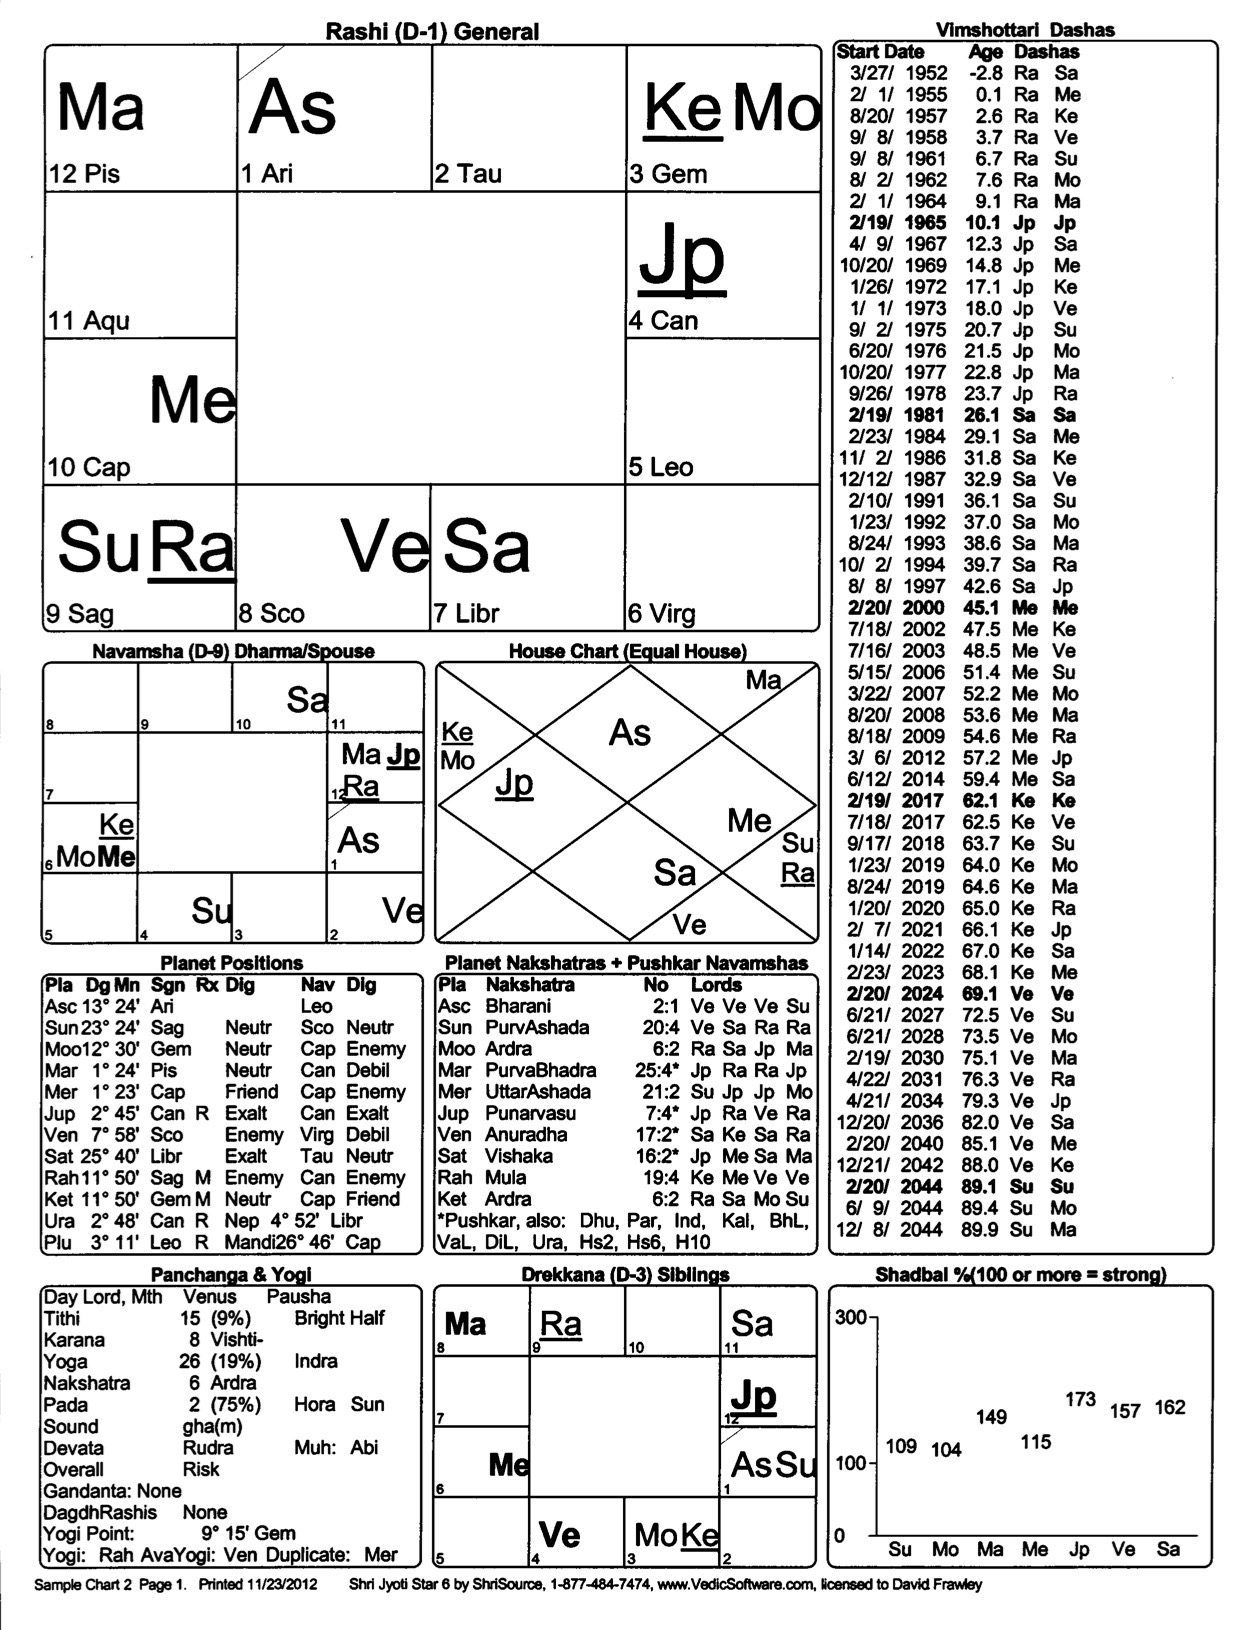
\includegraphics[width=10cm]{pics/lesson-2-Sample-Chart-2.jpeg}
\caption{}
\end{figure}


The chart is of a successful Yoga teacher, one who is highly educated, articulate, and a good therapist as well. It is an extraordinary chart in many respects with good outer and inner indications. The following chart shows many interesting and strong positions. See if you can identify them.

 
\begin{enumerate}
\item What planets are angular in the chart?
\item What planets occupy trines?
\item What planets occupy Duhsthanas?
\item What planets occupy upachaya houses?
\item What Mahapurusha Yogas are created in the chart?
\item Now examine the same positions from the Moon.
\item Now examine the same positions in the Navamsha.
\end{enumerate}

The chart has a strong Aries Ascendant endowing the native with initiative and leadership. Jupiter, the ninth and twelfth lords, ruling two spiritual houses, is located in the fourth house, a house of the heart and a Moksha house, where it is exalted created a Mahapurusha Yoga or Hamsa Yoga for Jupiter. This is very favorable for spiritual matters, for education, and for happiness in life.

 

However its retrograde status does spoil in somewhat though may aid the person spiritually, making him more introspective. In addition, Jupiter is strengthened by being vargottama (in the same sign in the birth and Navamsha charts).

 

 

Saturn is exalted in the seventh house as the tenth lord giving a powerful career status. It forms another Mahapurusha Yoga, that of Saturn or Shasha Yoga. Saturn also aspects Jupiter and both being in mutual angles affect each other. Such mutual angle relationships are often counted as a full aspect in Vedic Astrology. Jupiter spiritualizes the strong Saturn, while Saturn makes Jupiter more ascetic. Their relationship as ninth and tenth lords for Aries Ascendant constitutes a Raja Yoga.

 

Mercury, the indicator of the intellect and teaching, occupies the tenth house under the aspect of benefic Jupiter. It is also vargottama. This makes the person a Mercury type and gives him good intellectual abilities. Three of the four angles are occupied. Two by exalted planets and one by a benefic rendering the chart quite powerful.

 

The Sun, the benefic fifth lord, occupies the auspicious ninth house, and is surrounded on either side by benefics, Mercury and Venus (Shubhakartari Yoga). This raises the children of the native and increases both his intelligence and education (fifth house). The Sun is aspected by Saturn, rendering it more introspective, and by the full Moon, giving it charisma and compassion. Rahu is well placed with the Sun here and carries the influence of its exalted lord Jupiter. The nodes being direct give them yet more strength. Relative to the ninth house, the father of the native is also a very successful businessman.

 

The Moon, the fourth lord, occupies the third in Gemini, an upachaya house. While the third is not always the best house for the Moon because it can make it unstable, here the Moon is full making it quite strong. It has no malefic aspects but is with Ketu, which helps deepen the persons psychic insight. This Moon gives a very active and creative, though sometimes restless mind.

 

Yet the chart does have some significant Duhsthanas as well. Mars, the lord of the Ascendant is in the twelfth. However this is not at all bad. It is in Pisces, a sign of Jupiter aspected by an exalted Jupiter and having no other afflictions. This gives it a spiritualizing influence and helps the individual seek Moksha.

 

Venus, the lord of the second and seventh, is in the eighth house, another Duhshthana and is hemmed in between malefics (Papakartari Yoga), Sun-Rahu and Saturn. However it also has the trinal aspect of exalted Jupiter alleviating its affliction. This weak position of Venus as the seventh lord, along with Saturn in the seventh house, causes some strain to marriage but there are enough compensating factors to counter this and make the marriage endure.

 

Venus as a maraka can harm the health and longevity of the native. However fortunately for him the Venus Dasha does not begin until the year 2024, when he is 69 years old. Mars, the Lagna lord, though in the twelfth, has good aspects and the chart is otherwise strong. Hence this position is unlikely to harm the longevity of the person, though it will cause him to retire or be more of a hermit later on in life.

 

\subsubsection{Positions From the Moon}

Looking at the chart from the Moon in Gemini, the positions are also strong. Mars, the eleventh lord, occupies the tenth house, aspected by Jupiter the tenth lord. This gives Mars a strong tenth house influence, boosting the career, and diverts the usual negative effects of Mars for Gemini into a positive area. The Sun, the third lord, occupies the seventh, another angle and receives the aspect of the full Moon and exalted Saturn. An exalted Saturn occupies the fifth house, as the ninth lord, lord of another trine.

 

Jupiter, the seventh and tenth lord, is exalted in the second from the Moon, giving good powers of speech and a good income and also boosting the affairs of the seventh and tenth houses. The mutual aspect between Jupiter and Mercury as tenth lord and lord of the first from the Moon constitutes another Raja Yoga.

 

Venus and Mercury, two important planets for Gemini, however occupy Duhsthanas from the Moon, the sixth and the eighth. However both are aspected by Jupiter and Mercury has no malefic influences. This lends a spiritual and occult energy to Mercury and gives a profound mind. Venus suffers somewhat as the fifth and twelfth lord. The native only had one child (fifth house) late in life (Saturn).

 

\subsubsection{Positions from the Navamsha}

The Navamsha is dominated by angular planets from both the Ascendant and the Moon. Mars and Jupiter are present in the Lagna as the ninth and tenth lords, another Raja Yoga. The debility of Mars is cancelled by its association with exalted Jupiter. The aspect of the Moon, the lagna lord, contributes to this. Mercury joins the combination as the third and twelfth lord, perhaps adding more than detracting by his neutrality. However the lunar nodes do complicate the Yoga somewhat and give some strain to relationship. Saturns aspect, though not bad from the eleventh house, adds tension to the combination.

 

The fifth house is afflicted by the Sun and the aspect of Saturn but is compensated by the aspect of Jupiter. Venus suffers from debility and no positive aspects.

 

\subsubsection{Dashas and Bhuktis}

We will not examine this matter much in this lesson, which is aimed mainly at highlighting basic house and sign positions. However do look at the scheme of the Dashas.

 

The native was born under Rahu-Saturn. Jupiter Dasha commenced from the age of 10. Saturn Dasha began at the age of 26. Mercury Dasha begins at the age of 45. Ketu begins at the age of 62. Rahu in the ninth is not bad, since its lord is exalted. The Dashas of two exalted planets then follow and of three planets in angles (Jupiter-fourth, Saturn-seventh, and Mercury-ninth). Such a Dasha scheme is very favorable for the development of the native.

 

Saturns Dasha, though generally good, has had its complications. Saturn even when good causes us difficulties and delays that eventually become a source of greater growth. Saturn-Mars and Saturn-Rahu were difficult periods in this regard, which is not surprising given the malefic nature of these planets.

 

However Ketu and Venus Dashas can cause the native to retire more into the spiritual life and the Venus Dasha can result in health problems.

